\documentclass[a4paper,12pt]{article}
\usepackage{kotex}
\usepackage{geometry}
\geometry{
	total={150mm,237mm},
	left=30mm,
	top=30mm,
}
\usepackage{graphicx}
\graphicspath{ {./designs/} }
\usepackage{algpseudocode}
\usepackage{amsmath,amsfonts}
\usepackage{enumerate}

% simple commands---------------------------------------------
\newcommand{\abs}[1]{\left\vert#1\right\vert}
\newcommand{\set}[1]{\left\{#1\right\}}
\newcommand{\seq}[1]{\left<#1\right>}
\newcommand{\norm}[1]{\left\Vert#1\right\Vert}
\newcommand{\floor}[1]{\left\lfloor{#1}\right\rfloor}
%additional-------------------------------------------------------


\begin{document}
\begin{center}\LARGE
	\textbf{pixel world}
\end{center}
\vspace{0.5cm}
\hrule
\vspace{0.5cm}
\section{개요}
\subsection{기대 결과}\label{expected outcome}
2D 공간에 간단한 구조와 생태를 가진 생명체를 구현한다. 그 생명체에는 적절한 번식 및 진화 메커니즘이 있어서 세대가 지남에 따라 자연선택 및 성선택을 통한 진화가 일어난다. 진화한 생명체들에서는 실제 동물들에서도 보여지는 다양한 생존전략들 (e.g. 협력, 위장, 기생,..)이 발현된다. 
\subsection{지향점}\label{design philosophy} 
최소한의 구성요소만으로 가상공간에 동물계의 다양한 모습을 구현한다.
\subsection{기대 효과, 가능한 발전 방향}\label{future development}
\begin{itemize}
\item 흥미
\item multi sensory – multi output 인공지능 벤치마크 
\item 진화 알고리즘 또는 그것과 다른 인공지능 기법들과의 결합의 실험장 
\item 진화 및 진화심리학 모델들의 간접적 검증
\item 뇌 발달 이론들의 간접적 검증 
\item 효율적인 생명체를 만드는 인공지능 콘테스트  
\item 게임
\end{itemize}

\section{기본 세계관}
\subsection{구성요소}\label{world components}
물체(미니언,지물), 지형, 미네랄(동물성, 식물성), 영양, 색, 페로몬 

\subsection{이 해설서에서 쓸 용어들}\label{basic terms}
\begin{itemize}
\item 월드 : \ref{world components}의 구성요소들이 모두 들어있는 가상의 공간. 
\item 환경 : 월드의 구성요소 중 미니언이 아닌 모든 것들
\item 물체 : 미니언 또는 지물
\item 셀 : 정사각형 형태로, 월드를 이루는 공간의 기본 단위이다. 
\item 셀을 차지하다 : 물체의 일부가 감지될 수 있는 물리적 실체로써 그 셀에 존재하며 물리 법칙의 영향을 받는다. 
\item 셀을 차지하지 않는 상태 : 물체가 월드 상에 존재하나, 어떤 이유로 일시적으로 감지되지 않는 상태로 된 것.
\item 셀이 비어있다 : 그 셀을 차지하는 물체가 존재하지 않는다.  
\item 개체 : 개개의 미니언 
\item 모먼트 : 시간 단위. 미니언의 모든 행위와 여타 이벤트들은 시간 단위 마다 한번 씩 일어나게 된다.  
\end{itemize}

\subsection{미니언}\label{minion}
물체에 속한다. 
월드에서 태어나고, 죽고, 
감각 정보를 신경계를 통해 행위 정보로 변환하여 그 행위를 실행하고, 
소화, 배변, 죽음을 통한 사체 제공을 통해 생태계와 상호작용을 하고,
생식과 출산을 통해 종의 번영을 도모한다. 다음과 같은 기능들을 가진다. 
\begin{itemize}
\item 행위 : 
운동(\ref{jaw movement}), 턱운동(\ref{movement}), 페로몬 분비(\ref{emission})
\item 감각 :  
시각(\ref{visual input}), 후각(\ref{olfactory input})
\item 생태계와의 상호작용 :  
소화(\ref{digestion}), 배변(\ref{excretion}), 사망 (\ref{death})
\item 생식 관련 :  
성교(\ref{intercourse}), 임신(\ref{pregnancy}), 출산 (\ref{childbirth})
\end{itemize}

\subsection{지형}\label{geography}
셀을 차지하지 않으며, 미니언의 이동범위를 제한하거나 미니언에게 특정 영향을 끼친다. 
\ref{geography and stuff} 참조. 

\subsection{지물}\label{stuff}
물체에 속한다.
셀을 차지하며, 미니언의 이동 범위를 제한하거나 미니언에게 특정 영향을 끼친다. 
정지형. 운동형, 자유이동형이 있다. \ref{geography and stuff} 참조.

\subsection{미네랄 - 동물성}\label{animal mineral}
미니언의 사체에 해당한다. 
사망(\ref{death})을 통해 생성되며 소화(\ref{digestion})을 통해 소멸된다. 
셀을 차지하지 않는다. 

\subsection{미네랄 - 식물성}\label{plant mineral}
식물에 해당한다. 
영양에서의 전환(\ref{conversion})을 통해 생성되며 소화(\ref{digestion})을 통해 소멸된다. 
셀을 차지하지 않는다. 

\subsection{영양}\label{nutrition}
흙의 유기물에 해당한다.
배변(\ref{excretion})을 통해 생성되며 식물성 미네랄로의 전환(\ref{conversion})을 통해 소멸된다.
셀을 차지하지 않는다. 

\subsection{색}\label{color}
$(m,r,g,b)$ 네 축을 가지며 $(\floor{255*r},\floor{255*g},\floor{255*b})$는 시각화에서 보여지는 색의 rgb 값과 같으며, m은 미니언이 미네랄을 감지하게 하기 위해 도입된 새로운 축이다. 

\subsection{페로몬}\label{pheromone}
\ref{pheromone form} 참조.

\subsection{실제 세계와의 유사점}\label{similarity to real world}
\begin{itemize}
\item 질량 보존의 법칙이 성립한다. 이것은 미니언의 체력(\ref{hp}) 과 미네랄과 영양(\ref{mineral and nutrition})의 각 단위를 모두 (가령 1kg이라는) 등가로 이해했을 때의 얘기이다. 
\item 영양$\Rightarrow$미네랄 의 전환(\ref{conversion})은 일종의 주기적인 기후로 이해할 수 있다.  
\end{itemize}

\subsection{모먼트 당 연산순서}\label{computing order}
\begin{enumerate}
\item 모든 미니언의 운동 계획(\ref{move plan}) 도출 
\item 모든 미니언의 턱운동(\ref{jaw movement}) 시행, 그에 따른 결과 적용 
\item 모든 미니언의 운동(\ref{movement}) 시행, 그에 따른 결과 적용 
\item 미니언의 상태 변화 (나이++(\ref{age}), 배변(\ref{excretion}), 분비(\ref{emission}))  
\item 환경의 변화 
\item 학습(\ref{learning algorithm})
\end{enumerate}
%------------------------------------------------------------
\section{미니언}
\subsection{신체}\label{body}
\begin{figure}[h]
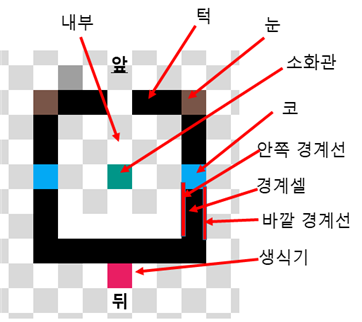
\includegraphics[scale=0.8]{minion_body_sample.png}
\centering
\caption{신체 샘플 이미지}
\label{figure:body}
\end{figure}
\subsubsection{용어}\label{body terms}
\begin{itemize}
\item 몸통 : 그림 \ref{figure:body}에서 검정색 영역을 모두 포함하는 최소의 직사각형 영역. 
\item 중심셀 : 몸통의 중심에 위치한 셀. 위 그림 \ref{figure:body} 소화관이 위치한 셀.
\item 가로 길이 : 몸통의 가로 길이 (홀수)
\item 세로 길이 : 몸통의 세로 길이 (홀수)
\item 면적 : (가로 길이)*(세로 길이)
\item 점유지 : 이 개체가 차지하는(\ref{basic terms}) 모든 셀들의 집합, 또는 그 개개의 셀. 위 그림에서 색칠되어 있는 셀들 중 소화관을 제외한 모든 곳.
\item 턱상태 : $(a,b)$ ($0\le a+b\le(\text{가로 길이})-2$) 인 정수 쌍. 양쪽 턱이 눈에서부터 얼마나 닫혀 있는지를 의미한다. 턱이 완전히 벌어진 상태는 $(0,0)$이고, 완전히 닫힌 상태에는 $a+b=(\text{가로 길이})-2$이 성립한다. 
\item 턱이 완전히 닫히다 : $a+b=(\text{가로 길이})-2$
\item 턱이 완전히 열리다 : $a+b=0$
\item 턱사이공간 : 양쪽 턱 사이의 $((\text{가로 길이})-2-a-b)$ 개 셀들이 있는 영역
\end{itemize}
\subsubsection{신체 사이즈 및 구성}\label{body size}
\begin{itemize}
\item 가로 길이 : 3 이상 31 이하의 홀수
\item 세로 길이 : 3 이상 31 이하의 홀수  
\item 눈, 코, 생식기는 항상 위 그림과 같은 배치를 가진다. (생식기의 길이가 달라질 수 있다는 점을 제외하고)
\item 생식기 길이 : $\floor{\max(1, C*sqrt(\text{면적}))}$ -- $C=0.2$
\item 소화관의 가로길이 :  $(\text{가로 길이})^C$ -- $C=0.6$
\item 소화관의 세로길이 :  $(\text{세로 길이})^C$ -- $C=0.6$
\newline(소화관은 셀을 차지하지는 않지만 이 크기는 \ref{digestion amount}의 소화량-소화관 크기 규칙에 의해 소화와 관련된다.)
\end{itemize}
\subsubsection{신체의 색}\label{body color}
\begin{itemize}
\item 모든 점유지는 색을 가진다. 
\item 눈과 코의 색은 모든 개체에서 동일하다. 
\item 생식기의 색은 하나의 형질이다. 
\item 눈, 코, 생식기 외의 점유지의 색은 하나의 형질이다.  
\end{itemize}

\subsection{형질}\label{trait}
개체간 차이를 만들어내는 개개의 특징을 의미한다.
\begin{itemize}
\item 외양 형질 : 가로 사이즈, 세로 사이즈, 생식기 색, 그 외 색(\ref{body color})
\item 신경 형질 : 신경계(\ref{brain})의 모든 매개변수들
\item 기타 형질 : 식성(\ref{taste}), 평균 자식수(\ref{pregnancy})
\end{itemize}
형질의 결정에 관해서는 \ref{heredity}을 참조. 

\subsection{생존지표 }\label{life indices}
\subsubsection{스태미나}\label{stamina}
운동(\ref{movement})과 턱운동(\ref{jaw movement})을 하는데 필요 
\begin{itemize}
\item 최대치 : $\floor{C*sqrt(\text{질량})}$ -- $C=10$
\item 소모 
\begin{itemize} 
\item 직진운동 : $\floor{C*\text{거리}}$ -- $C=1.0$
\item 후진운동 : $\floor{C*\text{거리}}$ -- $C=1.0$
\item 좌/우진운동 : $\floor{C*\text{거리}}$ -- $C=2.0$
\item 반시계/시계 회전운동 : $\floor{C*sqrt(\text{면적})}$  --$C=0.6$
\item 완전 회전운동 : $\floor{C*sqrt(\text{면적})}$ -- $C=1,0$
\item 턱운동 1회 시도: $\floor{C*sqrt(\text{면적})}$ -- $C=0.3$
\end{itemize}
\item 회복 : 모먼트 당 $\floor{C*sqrt(\text{면적})}$  --$C=0.8$
\end{itemize}
\subsubsection{체력(=질량)}\label{hp}
생존과 관련(\ref{death})되고 물리법칙(\ref{physics}) 등 개체와 환경의 각종 상호작용에 관여한다. 특히 최소치 이하가 되면 개체가 사망한다. 
질량 보존의 법칙(\ref{similarity to real world})을 위해 질량과 등가로 이해된다. 
\begin{itemize}
\item 최대치 : 100*(면적). 단 임신 시는 \ref{pregnancy} 참조 

\item 소모 :  배변(\ref{excretion}), 물리법칙(\ref{physics})에 의한 데미지 

\item 회복 : 소화(\ref{digestion})
\end{itemize}
\subsubsection{나이}\label{age}
0부터 시작하여 매 모먼트 마다 1씩 증가하며, 수명에 도달하면 개체가 사망한다. 
\begin{itemize}
\item 수명 결정 - 출산 시 $d$(-- $d\sim Poisson(1000)$)에 따라 결정된다.  
\end{itemize}

\subsection{성교, 임신, 출산, 사망} 
\subsubsection{성교}\label{intercourse}
\begin{itemize} 
\item 지속 중 효과 : 미정 
\item 개시 시 효과 : 그것을 일으킨 턱운동이 즉각 반려(III-5)되며, 확률 $p$(-- $p=1.0$)로 상대가 임신이 된다, 
\item 개시 조건 : 턱사이공간(\ref{body terms}) 셀 중 하나를 동종 타개체의 생식기가 차지하고 있고 나머지 셀들은 비어있을 때, 개체가 턱을 닫는 운동을 할 시 일어난다. 
\item 지속 :  0 모먼트 만에 끝이 난다. 
\end{itemize} 
\subsubsection{임신}\label{pregnancy}
\begin{itemize} 
\item 지속 중 효과 : 최대 체력이 출산예정자식들의 최대체력의 합만큼 늘어난다. 배변(\ref{excretion})이 되지 않는다. 개체는 자신의 임신여부를 지각(\ref{brain})한다. 
\item 개시 시 효과 : 출산예정자식수가 d(--d=Poisson(평균자식수(III-2)))에 따라 결정된다. 
\item 개시 조건 : 성교가 일어나고, 임신 확률읉 통과했을 때 
\item 지속 : 출산 시(정확히는 \ref{childbirth}의 가능한 시나리오 중 마지막이 일어날 때) 끝이 난다. 
\end{itemize}
\subsubsection{출산}\label{childbirth}
임신 중일 시, 소화를 통해 체력이 최대 체력에 도달했을 때 출산배치 규칙(\ref{childbirth arrangement})에 따라 출산이 일어난다. 그 결과는 세 가지 중 하나가 된다. 
\begin{itemize}
\item 자식들을 일부만 성공적으로 출산하고, 한명의 자식이 출산 중 사망하고, 출산예정자식수가 줄어든 상태로 임신 상태가 유지된다. 
\item 자식들을 모두 성공적으로 출산하고 임신 상태가 해제된다.  
\item 자식들을 전부 또는 일부 출산하고 출산 중 사망이 일어난다. 
\end{itemize} 
\subsubsection{사망}\label{death}
\begin{itemize}
\item 개시 시 효과 : 개체가 월드에서 삭제되며, 사망 직전 질량이 개체의 몸통이 있던 자리에 동물성 미네랄(\ref{animal mineral detail}) 균등하게 배분된다. 
\item 개시 조건 : 다음 경우 중 하나
\begin{enumerate}
\item 체력(\ref{hp})이 최소 체력 이하가 되었을 때
\item 나이(\ref{age})가 수명에 도달했을 때  
\end{enumerate}
\end{itemize} 

\subsection{운동 계획}\label{move plan}
매 모먼트가 시작할 때, 신경계(\ref{brain})를 통해 
운동계획이 수립된다. 이후 미니언마다 순차적으로 운동이  
수행되는데, 자신 외의 다른 미니언의 운동이 수행될 동안 이 계획은 변하지 않는다. 운동 계획의 종류로는 다음의 세 가지가 있다. 
\subsubsection{운동 타입}\label{move type}
정지, 평행운동(직진운동, 후진운동, 좌진운동, 우진운동),회전운동(반시계회전, 시계회전, 완전회전)의 8가지 종류 중 하나로 결정된다.
\subsubsection{운동 거리}\label{move distance}
0과 1 사이의 수로 결정되는데, 이는 최대 스태미나(\ref{stamina})에 대한 비율을 의미한다. 운동타입이 평행이동 중 하나일 때만 의미가 있다.
\subsubsection{턱운동 타입}\label{jaw movement type}
0, 1, 2 중 하나로 결정된다. 이것은 운동 횟수를 의미하며,
한번의 성공적인 운동은 턱을 완전히 열린 상태(\ref{body terms})에서 완전히 닫힌 상태(\ref{body terms}), 또는 완전히 닫힌 상태에서 완전히 열린 상태로 바꾼다.
\subsubsection{분비 페로몬}\label{emitting pheromone}
월드에 존재하는 페로몬(\ref{pheromone form}) 중 하나로 결정된다.


\subsection{운동, 턱운동}\label{movement and jaw movement}
\subsubsection{운동}\label{movement}
계획된 운동 타입(\ref{move type})과 운동 거리(\ref{move distance})를 기반으로 수행된다.
\begin{itemize} 
\item 정지 : 아무 일도 일어나지 않는다. 
\item 평행운동(d:이동거리) : 해당 방향으로 d번 질량 만큼의 힘(\ref{physics} 물리법칙 참조)을 가한다. 성공 시마다 스태미나가 소모된다. (\ref{stamina} 스태미나 참조) 
\item 회전운동 : 중심셀을 기준으로 한 회전을 의미한다. 운동 후 차지할 셀들이 모두 비어 있을 때만 운동이 시행되고, 그 외의 경우에는 운동이 반려된다. 운동이 시행 시 스태미나가 소모된다.(\ref{stamina} 스태미나 참조) 
\end{itemize}
\subsubsection{턱운동}\label{jaw movement}
계획된 턱운동 타입(\ref{jaw movement type})을 기반으로 수행된다. 
1번 턱운동을 시도할 때마다 스태미나가 소모된다. (\ref{stamina} 스태미나 참조)  
턱운동을 $n$($n=0,1,2$)번 시도할 때는 다음과 같은 일이 일어난다. 
\begin{itemize}
\item 0번의 턱운동을 시도하였을 때는 아무 일도 일어나지 않는다. 
\item 2번의 턱운동을 시도할 때는 1번의 턱운동을 시도한 후, 그것이 반려되었을 경우에는 멈추고, 성공하였을 때는 나머지 1번의 턱운동을 시도한다.
\item 턱이 완전히 닫힌 상태(\ref{body terms})에서 1번의 턱운동 시도할 경우, 턱이 완전히 열린다(\ref{body terms}). 이 때의 턱운동은 성공한 것으로 취급한다.  
\item 턱이 완전히 열린 상태(\ref{body terms})에서 1번의 턱운동 시도 
\begin{enumerate}
\item 성교의 조건(\ref{intercourse})이 만족되는 지 확인하고, 만족된다면 성교를 일으킨 후 턱운동을 반려한다. 그렇지 않는다면 (2)로 간다.
\item 개체를 정지형 지물로 일시적으로 지정(물리 법칙(\ref{physics})에 반영)한 후, 다음 과정을 턱이 완전히 닫히거나 턱운동이 반려될 때까지 반복하여 (a)를 시행한다. 턱이 완전이 닫힐 경우 운동이 성공한 것으로 취급하며 끝을 내고, 턱운동이 반려될 경우 (3)으로 간다. 
\begin{enumerate}
\item 좌측 턱이 막혀있을 경우 (b)로 간다. 그렇지 않을 경우 좌측 턱이 반대편으로 $\floor{C*\text{질량}}$ (-- $C=5.0$)만큼의 힘을 가한다(\ref{physics} 물리법칙 참조). 여기서 충돌이 일어났을 경우, 좌측 턱이 막힌 것으로 취급한다. 
\item 우측 턱이 반대편으로 int(C*질량) (--C=5.0)만큼의 힘(\ref{physics} 물리법칙 참조)을 가한다. 여기서 충돌이 일어났을 경우 턱운동을 반려시킨다.  
\end{enumerate}
\item 턱운동이 반려될 경우, 턱을 완전히 연다. 
\end{enumerate} 
\end{itemize}
이러한 운동의 실질적인 결과는 다음 중 하나로 나타난다.
\begin{itemize}
\item 성교가 일어나고, 턱이 완전히 열린 상태로 끝이 난다.
\item 턱사이공간(\ref{body terms}) 중에서도 불운한 위치에 있던 다른 미니언들이 데미지를 입고, 턱이 완전히 열린 상태로 끝이 난다. 
\item 단순히 턱의 상태만 완전히 열란 상태에서 완전히 닫힌 상태로, 또는 그 반대로 변화한다. 
\item 아무 일도 일어나지 않는다.
\end{itemize}

\subsection{소화, 배변}
\subsubsection{식성}\label{taste}
$0\sim 1$ 사이의 수로 동물성 미네랄과 식물성 미네랄의 소화 정도를 결정함. 0이면 완전한 초식동물, 1이면 완전한 육식동물로 생각할 수 있음.
\subsubsection{소화}\label{digestion}
\begin{itemize}
\item 개시 시 효과 : 소화량-소화관크기 규칙(\ref{digestion amount})에 따라 중심셀 근처의 각 셀의 미네랄 양에 맞춰 체력이 회복되며 동시에 그 셀들에서 해당하는 만큼의 미네랄이 감소된 후, 식성에 따라 즉각 설사량(다음 항목)만큼 배변이 일어난다. 
\item 개시 조건 : 매 모먼트 마다, 그리고 운동(\ref{movement})을 통해서든, 물리법칙(\ref{physics})을 통해서든 위치의 변화가 조금이라도 일어날 때마다 시행된다. 예를들어 2 이상의 거리만큼 평행운동 하는 경우에는, 한 셀 이동 할 때마다 소화가 일어난다.   
\end{itemize}
\subsubsection{설사량}\label{diarrhea amount}
$\floor{(\text{식성})*(\text{식물성 미네랄 소화량})+(1-(\text{식성}))*(\text{동물성 미네랄 소화량})}$
\subsubsection{배변}\label{excretion}
항상 배변량과 같이 주어지는데, 배변량 만큼 체력이 소모되며 그만큼의 영양(\ref{nutrition detail})이 생식기가 차지하는 셀들에 균등하게 분배된다. 다음 두가지 경우에 일어난다. 
\begin{itemize}
\item 매 모먼트 당 한번씩, 배변량 : $\floor{C*(\text{면적}))}$ -- $C=1.0$
\item 소화 직후, 배변량 : 설사량(\ref{diarrhea amount})
\end{itemize} 

\subsection{시각}\label{visual input}
\begin{itemize} 
\item 시력 : $(a,b)$ -- $a=88$, $b=88$
\item 시각 범위 : 몸통의 뒷부분부터 시작하는 $(3*(\text{가로사이즈}),3*(\text{세로사이즈}))$ 크기의 직사각형 영역 
\item 시각 인풋 : 월드의 이미지(\ref{rendering})를 시각 범위로 제한시킨 것을, 시력을 기준으로 해상도 조절한 것. 신경계(\ref{brain})의 인풋 중 하나로 쓰인다. 
\end{itemize}

\subsection{페로몬, 분비, 후각}
페로몬은 $n$ (-- $n=30$) 종류가 있으며 각 개체가 매 모먼트마다 운동 계획(\ref{emitting pheromone}동)에 따라 분비할 것을 결정하며, 후각을 통해 주변의 것들의 가중치 합을 감지한다.
\subsubsection{페로몬의 형태}\label{pheromone form}
$\in\mathbb{R}^n$ (-- $n=50$)
\subsubsection{분비}\label{emission}
운동 계획(\ref{emitting pheromone})을 기반으로 수행된다.
\subsubsection{후각}\label{olfactory input}
후각 인풋은 $self.smell=concat(\sum_{mi\neq self}\frac{mi.emission}{dist(self.nose1,mi.body)},\sum_{mi\neq self}\frac{mi.emission}{dist(self.nose2,mi.body)})$으로 결정된다. 
여기서 $dist(a,B)$는, 셀 $a$에서 셀 리스트 $B$ 까지의 최소의 $L^1$ 거리를 의미한다. 이것은 신경계(\ref{brain})의 인풋 중 하나로 쓰인다. 

\subsection{신경계}\label{brain}
\begin{itemize}
\item 인풋 : 후각, 시각, 체력, 스태미나, 임신 여부  
\item 아웃풋 : 운동타입(\ref{move type}), 운동거리(\ref{move distance}), 분비(\ref{emission})
\end{itemize}
신경계는 그림 \ref{figure:nn}의 도표와 같이 구성되며, 주목할 점은 단순한 피드포워드 네트워크가 아니라 '내적 상태'를 가진다는 것이다.
\begin{figure}[h]
	\centering
	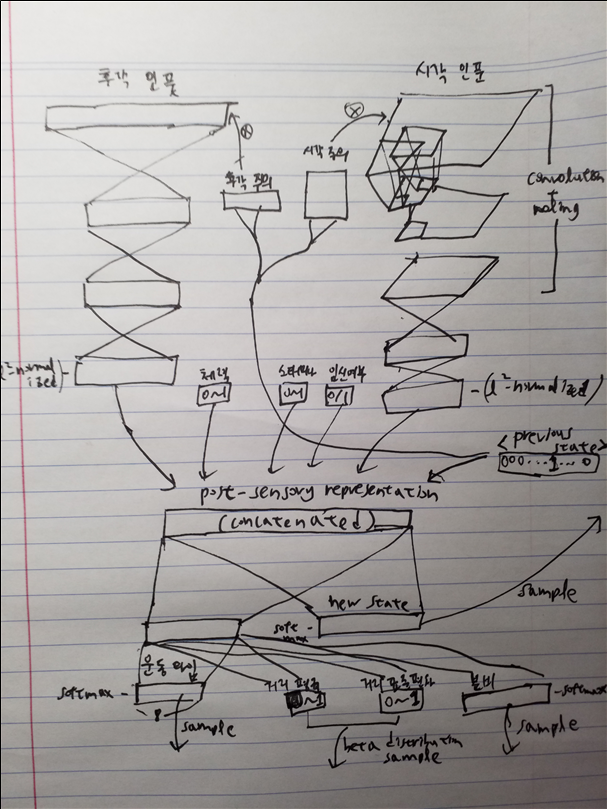
\includegraphics[scale=0.6]{minion_nn.png}
	\caption{신경계 구조}
	\label{figure:nn}
\end{figure} 

\subsection{종, 유전}\label{heredity}
\begin{itemize} 
\item 정의 : 현재 버전에서는 고정된 리스트의 ‘종’이 있으며 어떤 종의 모든 개체는 모든 형질을 공유한다. 
\item 종과 형질의 결정 : 현재 버전에서는 새로 출생한 개체의 종은 부모의 것과 같아진다. 
\item 후생 유전 : 현재 버전에서는 학습(\ref{heredity})을 통해 어떤 종의 신경 형질이 매 모먼트마다 변화한다.
\end{itemize} 
%------------------------------------------------------------

\section{지형 지물}\label{geography and stuff}
\subsection{지형의 분류}\label{geography classification} 
미정
\subsection{지물의 분류}\label{stuff classification}
\begin{itemize} 
\item 정지형 지물
\item 운동형 지물 : 물리 법칙에 영향을 받지 않고 확정적으로 운동을 함.
\item 자유이동형 지물 : 질량을 가지고 물리 법칙에 따라 이동함.
\end{itemize} 
\subsection{정지형 지물의 종류}\label{immobile stuffs}
\begin{itemize} 
\item 월드의 바깥 경계 : (물리 법칙(\ref{physics})과 관련해서 편의 상 정지형 지물로 생각한다.) 색은 $(0,1,0,0)$이다.(빨강으로, 모티브는 불지옥이다.)
\end{itemize}
\subsection{운동형 지물의 종류}\label{mobile stuffs}
미정
\subsection{자유이동형 지물의 종류} \label{free-moving stuffs}
미정
%--------------------------------------------------------

\section{미네랄 및 영양}\label{mineral and nutrition}
미네랄과 영양은 모두 셀마다 부여된 음이 아닌 정수 값으로 셀을 차지하지 않지만, 이 중 미네랄은 색(\ref{color})으로 나타난다. 
\subsection{동물성 미네랄}\label{animal mineral detail}
생성 : 사망(\ref{death})
소멸 : 소화(\ref{digestion}) 

\subsection{식물성 미네랄 }\label{plant mineral detail}
\begin{itemize} 
\item 생성 : 영양에서의 전환(\ref{conversion})
\item 소멸 : 소화(\ref{digestion})
\end{itemize}

\subsection{영양}\label{nutrition detail}
\begin{itemize}
\item 생성 : 배변(\ref{excretion})
\item 소멸 : 식물성 미네랄로의 전환(\ref{conversion})
\end{itemize}  

\subsection{영양$\Rightarrow$식물성 미네랄 전환}\label{conversion}
$T$ (-- $T=30$)모먼트에 한번 씩 각 셀의 모든 영양이 같은 숫자의 식물성 미네랄로 전환된다.

\subsection{미네랄의 색}\label{mineral color}
$(\tanh((\text{동물성}+\text{식물성})/C),\tanh(\text{동물성}/C),\tanh(\text{식물성}/C),0)$ (-- $C=100$)

%----------------------------------------------------------
\section{물리법칙}\label{physics}
운동형 지물 또는 미니언인 $A$가 방향 $d$로 $F$만큼의 힘을 가했다고 하면 다음의 일이 일어난다. 
\begin{enumerate}
\item $l$을 ($A$가 $d$쪽으로 한칸 움직였을 때의 점유지)$\setminus$($A$의 점유지)  (차집합)에 해당하는 셀들의 집합이라고 하자. 
\item $l$의 모든 셀들이 비어있으면, $A$를 $d$쪽으로 한칸 이동시키고 끝이 난다. 
\item 그렇지 않으면 “$A$에 의해 힘을 받는 모든 물체들”(미니언과 자유이동형 지물들로 이루어짐)의 집합 $B$와 “충돌”이 발생하는지의 여부를 동시에 계산한다.
\item 만약 충돌이 발생하지 않고 $B$의 모든 물체의 질량이 합이 $F$보다 크면, 아무 일도 일어나지 않고 끝이 난다. 
\item 만약 충돌이 발생하지 않고 $B$의 모든 물체의 질량의 합이 $F$ 이하이면, $A$와 $B$의 물체들 모두를 $d$ 방향으로 한칸 이동시키고 끝이 난다. 
\item 만약 충돌이 발생하면, $B$의 물체들 중 미니언인 것들은 모두 $F$만큼의 체력 소모가 생긴다. 
\end{enumerate}

“$A$에 의해 힘을 받는 모든 물체들” 과 “충돌” 여부는 그림 \ref{figure:move1}, \ref{figure:move2}, \ref{figure:move3}에서와 같이 계산된다. "충돌"이 발생한 경우 "힘을 받는 물체들"은 현실상황이라면 압사당할 위기에 놓인 물체들이라고 할 수 있다.
\begin{figure}[h]
	\centering
	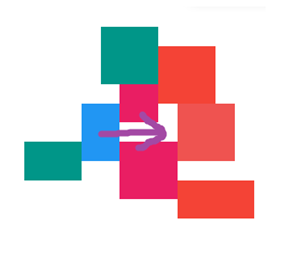
\includegraphics[scale=0.9]{move1.png}
	\caption{ 파란색은 힘을 가하는 주체를, 빨간색 계열은 그것에 의해 힘을 받는 물체(미니언 또는 자유이동형 지물)들을, 검정색은 충돌 여부를 결정짓는 정지형 또는 운동형 지물을, 초록색 계열은 현재 상황에서 힘을 받지 않는 그 외의 물체(미니언 또는 자유이동형 지물)을 의미한다. 이 경우는 충돌이 발생하지 않았다.}
	\label{figure:move1}
\end{figure} 
\begin{figure}[h]
	\centering
	
\includegraphics[scale=0.7]{move2.png}
	\caption{ 파란색은 힘을 가하는 주체를, 빨간색 계열은 그것에 의해 힘을 받는 물체(미니언 또는 자유이동형 지물)들을, 검정색은 충돌 여부를 결정짓는 정지형 또는 운동형 지물을, 초록색 계열은 현재 상황에서 힘을 받지 않는 그 외의 물체(미니언 또는 자유이동형 지물)을 의미한다. 이 경우는 충돌이 발생했다.}
	\label{figure:move2}
\end{figure} 
\begin{figure}[h]
	\centering
	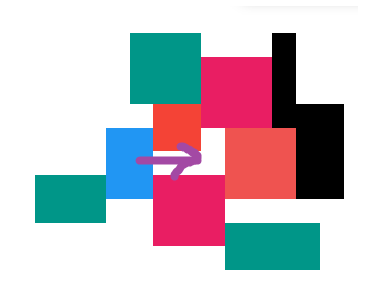
\includegraphics[scale=0.7]{move3.png}
	\caption{ 파란색은 힘을 가하는 주체를, 빨간색 계열은 그것에 의해 힘을 받는 물체(미니언 또는 자유이동형 지물)들을, 검정색은 충돌 여부를 결정짓는 정지형 또는 운동형 지물을, 초록색 계열은 현재 상황에서 힘을 받지 않는 그 외의 물체(미니언 또는 자유이동형 지물)을 의미한다.이 겨우는 충돌이 발생했다.}
	\label{figure:move3}
\end{figure} 

%---------------------------------------------------------------

\section{렌더링}\label{rendering}
월드의 구성요소들의 현재 상태롤 통해 각 셀을 색(\ref{color})으로 대응시키는 함수를 계산하는 과정. 렌더링 된 결과를 ‘월드의 이미지’라고 할 것이다. 
\subsection{렌더링 규칙}\label{rendering rule}
어떤 셀에 대하여,
\begin{enumerate} 
\item 그 셀을 차지하는 미니언 또는 지물이 있으면, 그 셀의 색은 미니언(\ref{body color}) 또는 지물(\ref{immobile stuffs},\ref{mobile stuffs},\ref{free-moving stuffs}) 항목에서 그것의 점유지의 색의 지정한 것을 따른다.  
\item 그렇지 않은 경우에는 미네랄에 의해 지정된 색(\ref{mineral and nutrition})에 지형에 의한 효과(\ref{geography classification})를 적용한 것이 그 셀의 색이 된다.  
\end{enumerate}

%------------------------------------------------------------

\section{학습 알고리즘}\label{learning algorithm}

현재 버전에서는 강화학습을 통해서만 학습을 한다. 
강화학습의 상황을 다음과 같이 정의한다.
\begin{itemize}
	\item 상태(state) – 이전 내적 상태 + 인풋 
	\item 액션(action) – 새로운 내적 상태 + 아웃풋
	\item 보상(reward) – 이후 $0\sim t$ (--$t=100$) 모먼트 까지의 평균 ‘종 적합도’ 
\end{itemize}
여기서 샹태(state)와 액션(action)을 이렇게 정의한 이유는,
그림 \ref{figure:nn}의 신경계 도표에서 볼 수 있듯이 신경계가 모든 인풋에 같은 아웃풋을 내는 것이 아니라 그 과정이 내적 상태에도 의존하기 때문이다. 
여기서 ‘종 적합도’란 해당 종의 모든 개체들의 체력(\ref{hp})의 합을 의미한다. 
\par 
이러한 세팅에서 일종의 정책 그라디언트(policy gradient) 방법에 일종의 복기 기억 (replay memory, https://arxiv.org/abs/1312.5602)을 적용한 것을 이용한다. 복기 기억의 용량은 위의 $t$ 값으로 한다. 한번의 학습 과정을 요약하면 다음과 같아지고, 이것을 매 모먼트 마다 시행(\ref{computing order})한다. 


\begin{algorithmic}
\State $loss\gets 0$
\ForAll {minion of species X}
	\State 
	\begin{enumerate}
	\item$minion$의 복기 기억에 직전 계산에서의 (이전 상태, 인풋, 이후 상태, 아웃풋)을 추가한다. 
	(길이가 $t$(-- $t=100$)이 넘어가면 가장 먼저 들어간 기억을 삭제한다.)
	\item $minion$의 복기 기억에서 $(ps,i,ns,o)$를 랜덤으로 선택한다.
	\item $loss+=(\text{현재 신경계의 매개변수 값들에서} (ps,i)\text{의 상태에서}$\newline $(ns,o)\text{의 액션을 취할 확률})$(연속 분포에 대해서는 확률밀도함수를 이용한다.)
	\end{enumerate}
\EndFor 
\State $loss\gets(X\text{의 종 적합도})*loss$ 
\State $(parameters)\gets(parameters)-\alpha\nabla loss$
\end{algorithmic}

%-------------------------------------------------------------

\section{기타 기술적인 규칙}
\subsection{출산배치 규칙}\label{childbirth arrangement}
$A$가 $B_1$,...,$B_n$ ($n$은 $A$의 출산 예정 자식 수)을 출산할 때는 다음과 같은 순서를 따른다.도
\begin{enumerate}
\item 일시적으로 $A$를 셀을 차지하지 않는 상태로 바꾼다. 
\item 각 $i=1,2,\cdots,n$ 에 대해 다음을 시행한다. 
\begin{enumerate}
 \item 
 $A$의 출산예정자식수를 1 감소시키고, 체력을 $(B_i\text{의 체력})+(\text{(출산시출혈량)})$ (--$(\text{출산시출혈량})=10*(\text{면적})$)만큼 감소시킨다.  
 $B_i$를 최대 체력을 가진 상태로 만든 다음, $B_i$를 $A$의 중심셀로 위치시킬 수 있는 지 확인한다.
\item 셀들이 모두 비어있지 않아 이동이 불가능 할 시, $B_i$는 사망하고 (3)으로 간다.
\item 이동이 가능할 시 $B_i$를 해당 자리에 위치시킨 다음, $B_i$가 랜덤한 방향으로 $(\text{해당 방향으로의 길이})*2$ 횟수만큼 막강한 힘 $F$(-- $F=1000*(\text{질량})$)를 가한다. (\ref{physics} 물리법칙 참조) 대부분의 경우 $B_i$는 이후의 자식들이 태어날 자리가 생길 만큼 충분히 멀어진다. 

\end{enumerate}
\item $A$의 출산 예정 자식 수가 0인 상태라면, $A$를 임신하지 않은 상태로 바꾼다. $A$를 다시 셀을 차지하는 상태로 바꾸려고 한다. 
\item $A$가 있던 자리의 셀들이 하나라도 비어있지 않을 시, $A$는 사망한다. (‘출산 중 사망’)
\item $A$가 있던 자리의 셀들이 모두 비어있을 시, $A$를 다시 셀을 차지하는 상태로 바꾼다. 
\end{enumerate}

\subsection{소화량-소화관크기 규칙}\label{digestion amount}
소화관은 직사각형 모양의 영역이며 그 중심이 개체의 중심셀에 위치한다고 생각한다. 그렇게 하였을 때 어떤 셀이 
\begin{enumerate}
\item 소화관에 의해 완전히 덮힌다면, 
현재 셀에 있는 (식물성 미네랄,동물성 미네랄)이 남김없이 최대한 소화된다. 최대 최력을 넘어서 일부만 소화될 시 원래 셀에 있던 비율에 맞춰서 소화된다. 
\item 소화관에 의해 완전히 덮히지 않는다면, 
\begin{enumerate} 
\item 그 셀이 소화관에 의해 덮여지는 비율 p를 계산한다. 
\item 셀이 소화관의 가로 모서리의 일부라면, 소화 비율 q=p/(개체의 세로 길이)를 계산한다. 그게 아니고 셀이 소화관의 세로 모서리의 일부라면, 소화 비율 q=p/(개체의 가로 길이)를 계산한다. 
\item 현재 셀에 있는 (식물성 미네랄,동물성 미네랄)이 비율 q에 해당하는 만큼만 최대한 소화된다. 최대 체력을 넘어서 일부만 소화될 시 원래 셀에 있던 비율에 맞춰서 소화된다. 
\end{enumerate}
\end{enumerate}

\end{document}